\scanpage{11}
\mspage{3}
% Header: one upper and three lower physical text baselines, plus the arrow/sign band.
% The doubtful comma represents the detached curve before combinatoires; its physical attachment is open.
\diagram{\begin{tikzcd}[row sep=huge]
{\text{``Arbres plans''}\text{\rlap{\raisebox{1.8ex}{\inserted{(non ponctuels)}}}}\text{ (dans un plan pas néc. \deleted{orienté})}}\arrow[d,leftrightarrow,"\approx",to path={([xshift=-4cm]\tikztostart.south)--([xshift=-4cm]\tikztotarget.north)\tikztonodes}]\\
{\begin{gathered}\text{polygônes\unsure{,} combinatoires, avec \deleted{\unsure{involution|relation}} inv. sans}\\\text{pts fixes non pénétrante sur l'ens des}\\\text{\deleted{\unsure{sommets}}\inserted{\unsure{arêtes|côtés}.}}\end{gathered}}
\end{tikzcd}}
\par\noindent\rule{\linewidth}{.4pt}

% L01
Revenant au cas d'un graphe $\Gamma$ circularisé \inserted{général},
% L02
Topologiquement, le graphe top. $|\Gamma|$
% L03
se déduit de $|C|$ par \deleted{\unsure{les identifications}}
% L04
\unsure{un|i.e.} quotient par \unsure{la|C} relation d'%
% L05
équivalence suivante : on recolle
% L06
l'arête $a$ et l'autre $\unsure{\sigma_C a|\sigma_C^a}$, en \uline{renversant} les
% L07
orientations induites sur ces \unsure{arêtes|côtés}.

% L08
Dans le cas où $\Gamma$ est un
% L09
arbre, on peut interpréter
% L10
celui-ci \inserted{top.${}^{t}$} en considérant
% L11
$C$ comme le bord
% L12
d'un disque orienté $D$,
% L13
subdivisé en \unsure{arêtes|côtés}, et
% L14
en joignant les ``centres''
% L15
des \unsure{arêtes|côtés} qui se correspondent
% L16
par $\sigma_C$, de façon à ce que les seg-\linebreak
% L17
ments obtenus ne se rencontrent pas.

\figure{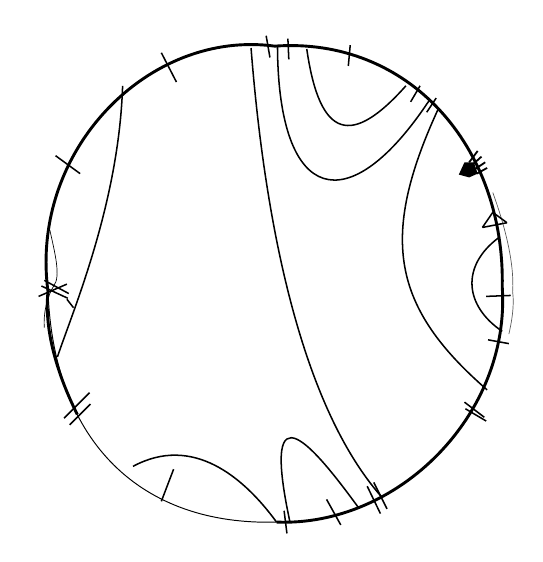
\begin{tikzpicture}[x=.012cm,y=-.012cm,line width=.55pt]
% F01 Thin continuous boundary, including thin lower-left arc
\draw[line width=.35pt] (95,1640).. controls (75,1490) and (202,1362)..(335,1380).. controls (476,1370) and (579,1485)..(576,1635).. controls (585,1770) and (466,1889)..(337,1884).. controls (194,1888) and (101,1800)..(95,1640);
% F02 Heavier retraced left, upper, right and lower-right boundary
\draw[line width=1.05pt] (126,1770).. controls (102,1722) and (91,1676)..(95,1640).. controls (75,1490) and (202,1362)..(335,1380).. controls (476,1370) and (579,1485)..(576,1635).. controls (585,1770) and (466,1889)..(337,1884);
% F03 Thin outer return beside heavy right rim; local ends approximate
\draw[line width=.25pt,black!65] (566,1535).. controls (579,1571) and (589,1610)..(587,1640).. controls (589,1655) and (586,1672)..(583,1685);
% F04 Interior curve1 close to left rim
\draw (174,1422).. controls (170,1547) and (121,1661)..(105,1709);
% F05 Interior curve2 long upper-to-lower-right span
\draw (310,1382).. controls (326,1586) and (368,1766)..(448,1857);
% F06 Interior curve3 larger upper-right nested cup
\draw (338,1381).. controls (339,1547) and (413,1567)..(499,1437);
% F07 Interior curve4 smaller upper-right cup
\draw (369,1383).. controls (383,1480) and (417,1486)..(474,1422);
% F08 Interior curve5 bowed left from right rim
\draw (508,1447).. controls (445,1584) and (460,1657)..(560,1744);
% F09 Interior curve6 small middle-right cup
\draw (572,1583).. controls (532,1613) and (536,1655)..(576,1682);
% F10 Interior curve7 low bottom-left arch
\draw (185,1825).. controls (248,1791) and (302,1836)..(337,1884);
% F11 Interior curve8 small upright bottom arch
\draw (351,1883).. controls (319,1733) and (378,1806)..(424,1869);
% F12 Single oblique crossing tick
\draw (215,1387)--(231,1418);
% F13 First short near-vertical top tick
\draw (326,1369)--(330,1392);
% F14 Second short near-vertical top tick
\draw (349,1372)--(350,1394);
% F15 Single near-vertical tick
\draw (415,1379)--(413,1401);
% F16 First tick crossing rim obliquely
\draw (479,1439)--(489,1422);
% F17 Second tick crossing rim obliquely
\draw (496,1450)--(506,1435);
% F18 Merged dark inner part of four-pronged hatch; no inferred four full crossings
\fill (530,1516)--(536,1503)--(546,1503)--(550,1515)--(541,1519)--cycle;
% F19 Visible outward prong, inner end merged into F18
\draw[line width=.65pt] (541,1503)--(550,1491);
% F20 Visible outward prong, inner end merged into F18
\draw[line width=.65pt] (543,1507)--(554,1497);
% F21 Visible outward prong, inner end merged into F18
\draw[line width=.65pt] (546,1511)--(558,1503);
% F22 Visible outward prong, inner end merged into F18
\draw[line width=.65pt] (549,1515)--(560,1509);
% F23 First edge of triangular mark
\draw (555,1572)--(581,1567);
% F24 Second edge of triangular mark
\draw (581,1567)--(566,1556);
% F25 Third edge closing triangular mark
\draw (566,1556)--(555,1572);
% F26 Transverse tick
\draw (559,1645)--(585,1644);
% F27 Transverse tick
\draw (561,1691)--(583,1695);
% F28 First trace of paired mark
\draw (536,1757)--(557,1773);
% F29 Second trace of paired mark
\draw (537,1764)--(559,1777);
% F30 First trace of paired mark
\draw (433,1846)--(447,1875);
% F31 Second trace of paired mark
\draw (440,1842)--(454,1870);
% F32 Single oblique bottom tick
\draw (390,1860)--(405,1887);
% F33 Near-vertical bottom tick
\draw (345,1872)--(348,1896);
% F34 Oblique tick on thin arc
\draw (228,1828)--(215,1862);
% F35 First close trace of paired mark
\draw (112,1774)--(139,1747);
% F36 Second close trace of paired mark
\draw (118,1781)--(140,1759);
% F37 First crossing stroke
\draw (85,1645)--(115,1632);
% F38 Second crossing stroke
\draw (88,1634)--(116,1647);
% F39 Third crossing stroke
\draw (91,1628)--(117,1642);
% F40 Detached short oblique fragment
\draw (115,1648)--(122,1657);
% F41 Single crossing tick
\draw (103,1496)--(129,1515);
% F42 Thin parallel returning trace beside heavy rim and hatch; ends approximate
\draw[line width=.25pt] (97,1575).. controls (102,1598) and (109,1624)..(101,1634).. controls (94,1645) and (90,1663)..(91,1678);
\end{tikzpicture}}

% L18
Les sommets de $\Gamma$ correspondent alors
% L19
aux régions découpées dans $D$, et les arêtes
% L20
orientées de $\Gamma$ aux frontières communes orientées,
% Thin grey other-hand foliation.
\margin{10}
